\chapter{Конструкторская часть}

В данном резделе будут представлены схемы алгоритмов умножения матриц,
приведены оценки трудоемкости алгоритмов.

\section{Представление алгоритмов}

На рисунках \ref{fig:images-winograd1} --- \ref{fig:images-winograd2} представлен классический
алгоритм умножения матриц. На рисунках \ref{fig:images-winograd1} ---
\ref{fig:images-winograd22} представлены два алгоритма умножения матриц Винограда ---
обычный и оптимизированный.

\begin{figure}[h]
    \centering
    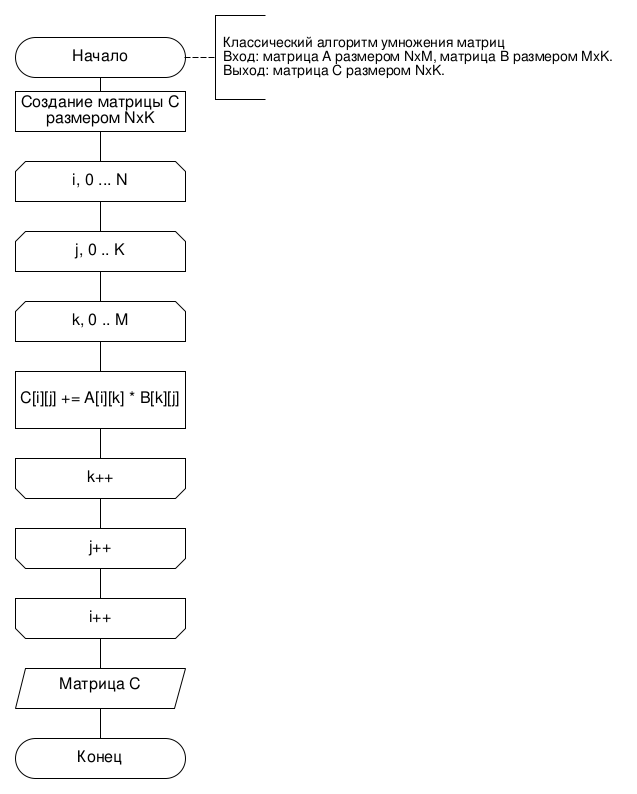
\includegraphics[width=0.6\textwidth]{images/classic}
    \caption{Классический алгоритм умножения матриц}
    \label{fig:images-classic}
\end{figure}

\clearpage

\begin{figure}[h]
    \centering
    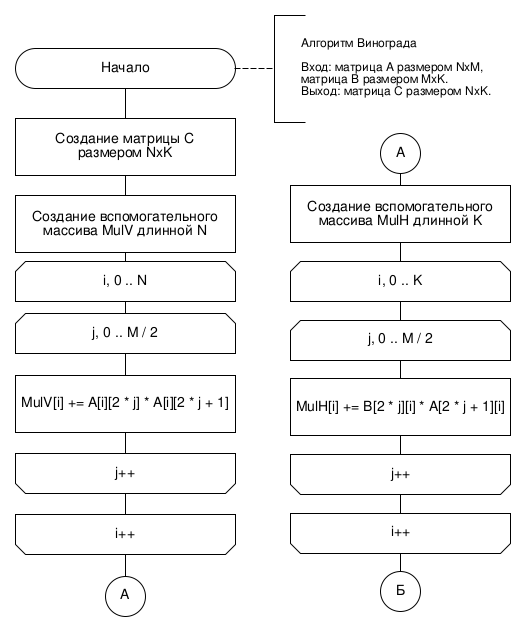
\includegraphics[width=0.8\textwidth]{images/winograd1}
    \caption{Алгоритм Винограда. Часть 1}
    \label{fig:images-winograd1}
\end{figure}

\clearpage

\begin{figure}[h]
    \centering
    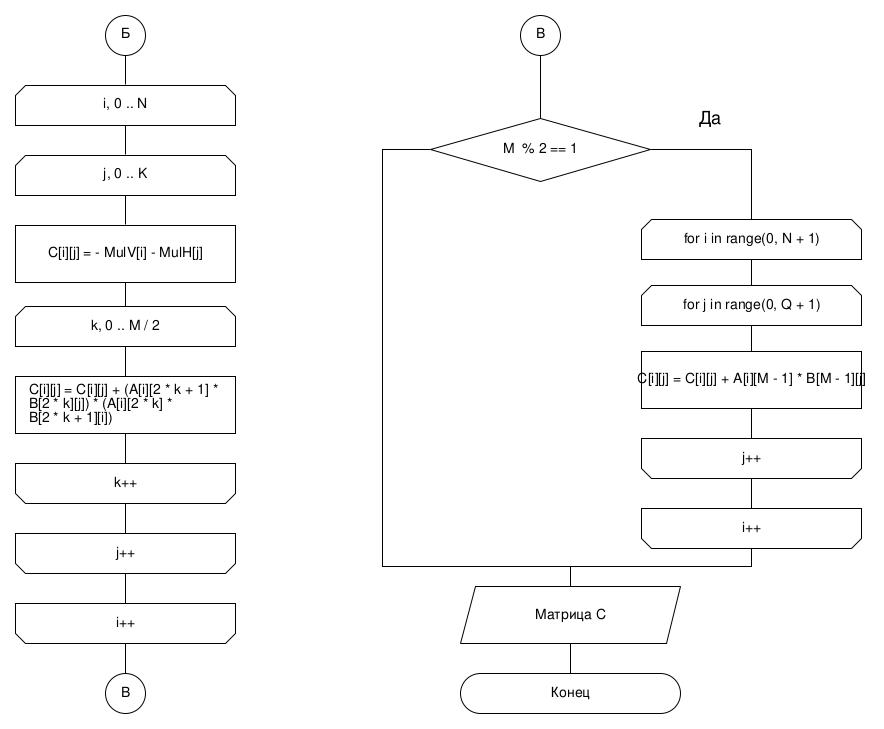
\includegraphics[width=0.8\textwidth]{images/winograd2}
    \caption{Алгоритм Винограда. Часть 2}
    \label{fig:images-winograd2}
\end{figure}




\begin{figure}[h]
    \centering
    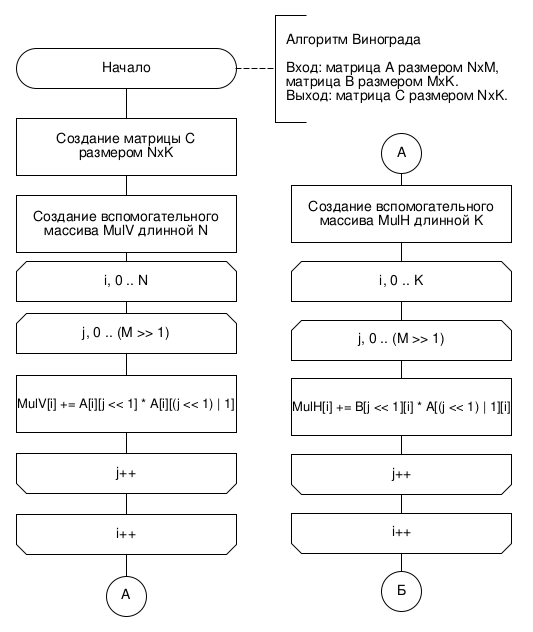
\includegraphics[width=0.8\textwidth]{images/winograd11}
    \caption{Оптимизированный алгоритм Винограда. Часть 1}
    \label{fig:images-winograd11}
\end{figure}

\clearpage

\begin{figure}[h]
    \centering
    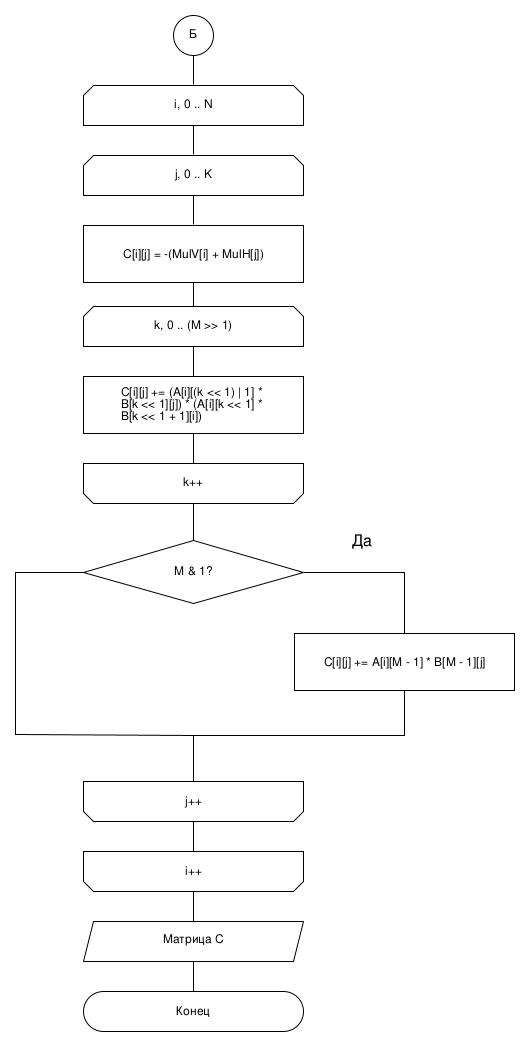
\includegraphics[width=0.6\textwidth]{images/winograd22}
    \caption{Оптимизированный алгоритм Винограда. Часть 2}
    \label{fig:images-winograd22}
\end{figure}

\clearpage


\subsection{Трудоемкость алгоритмов}

В следующих подразделах будут рассмотрены трудоемкость алгоритмов
умножения матриц.
Во всех последующих алгоритмах не будем учитывать инициализацию
матрицы, в которую записывается результат, потому что данное действие
есть во всех алгоритмах. Размер матрицы $A$  $N\times M$, размер матрицы $B$  $M\times K$.


\subsection{Модель вычислений}


Следующие операции будут иметь трудоемкость 1:
\begin{equation}
    +,-,[ \  ], <<, >>, |, &, <, <=, >, >=, =, ==, ++, --, +=, -=
\end{equation}

Следующие операции будут иметь трудоемкость 2:
\begin{equation}
    *, /, \%, *=
\end{equation}

Трудоемкость цикла будет рассчитываться как:
\begin{equation}
    f_{cycly} = f_{init} + f_{check} + N(f_{body} + f_{check}),
\end{equation}
где $N$ - количество итераций цикла.

\medskip

Трудоемкость условного оператора будет определяться как:
\begin{equation}
    f_{if} = \begin{cases}
        f_{check}, & $ трудоемкость в случае невыполнения условия, \\
        f_{check} + f_{body}, & $ иначе.
    \end{cases}
\end{equation}

\subsection{Классический алгоритм}

Трудоемкость
\begin{itemize}
    \itemm внешнего цикла $i = \overline{1,N}$:
    \begin{equation}
        f_i = 2 + N\cdot (f_{ibody} + 2);
    \end{equation}
    \itemm внутреннего цикла $j = \overline{1,K}$:
    \begin{equation}
        f_{ibody} = 2 + K \cdot (f_{jbody} + 2);
    \end{equation}

    \itemm внутреннего цикла $k = \overline{1, M}$:
    \begin{equation}
        f_{jbody} = 2 + M \cdot (12 + 2);
    \end{equation}
\end{itemize}

Тогда, если объединить (2.1) --- (2.3):
\begin{equation}
    f = 2 + N \cdot
    (
        4 + K \cdot
        (
            4 + 14M
        )
    );
\end{equation}

После упрощения (2.8):
\begin{equation}
    f = 14NKM + 4NK + 4N + 2 \approx 14NKM.
\end{equation}


\subsection{Алгоритм Винограда}

Трудоемкость
\begin{itemize}
    \itemm создания и инициализации массивов $MulH$ и $MulV$:
    \begin{equation}
        f_{init} = M + N;
    \end{equation}

    \itemm Заполнения массива $MulH$:
     \begin{equation}
        f_H = 2 + N(2 + \frac{M}{2}\cdot 17);
    \end{equation}

    \itemm Заполнения массива $MulV$:
     \begin{equation}
        f_V = 2 + K(2 + \frac{M}{2}\cdot 17);
    \end{equation}

    \itemm основного цикла умножения для четных размеров матриц:
    \begin{equation}
        f_{cycle} = 2 + N(2 + K(11 + 14M));
    \end{equation}

    \itemm цикла умножения последней нечетной строки и последнего нечетного столбца:
    \begin{equation}
        f_{odd} = \begin{cases}
            2, & $четный размер\\
            2 + N(2 + 14K), & $иначе
        \end{cases}
    \end{equation}.
\end{itemize}

Для нечетной размерности матрицы трудоемкость:
\begin{equation}
    f_{1} = f_{init} + f_H + f_V + f_{cycle} + f_{odd} \approx 14NMK.
\end{equation}


\subsection{Оптимизированный алгоритм Винограда}

Трудоемкость
\begin{itemize}
    \itemm создания и инициализации массивов $MulH$ и $MulV$:
    \begin{equation}
        f_{init} = M + N;
    \end{equation}

    \itemm Заполнения массива $MulH$:
     \begin{equation}
        f_H = 2 + N(2 + \frac{M}{2}\cdot 11);
    \end{equation}

    \itemm Заполнения массива $MulV$:
     \begin{equation}
        f_V = 2 + K(2 + \frac{M}{2}\cdot 11);
    \end{equation}

    \itemm цикл умножения для четных размеров матриц:
    \begin{equation}
        f_{cycle even} = 2 + N(2 + K(11 + 8.5\cdot M));
    \end{equation}

    \itemm цикл умножения для нечетных размеров матриц:
    \begin{equation}
        f_{cycle odd} = 2 + N(2 + K(22 + 8.5\cdot M));
    \end{equation}

\end{itemize}

Для нечетной размерности матриц трудоемкость:
\begin{equation}
    f_{1} = f_{init} + f_H + f_V + f_{cycle odd} \approx 8.5\cdot NMK.
\end{equation}

\paragraph*{ВЫВОД} ${}$ \newline

В данном разделе были рассмотрены представления алгоритмов и трудоемкость их выполнения.
Классический алгоритм и обычный алгоритм Винограда имеют одинаковую трудоемкость.
Оптимизированный алгоритм Винограда имеет наименьшую трудоемкость из представленных алгоритмов.

